\documentclass[12pt,a4paper]{report}
\usepackage[utf8]{inputenc}
\usepackage[T1]{fontenc}
\usepackage[english]{babel}
\usepackage[top=2.5cm,bottom=2.5cm,left=2.5cm,right=2.5cm]{geometry}
\usepackage{amsmath,amssymb,amsthm}
\usepackage{graphicx}
\usepackage{tikz}
\usepackage{pgfplots}
\pgfplotsset{compat=1.18}
\usepackage{tcolorbox}
\usepackage{enumitem}
\usepackage{hyperref}
\usepackage{bookmark}
\usepackage{fancyhdr}
\usepackage{titlesec}

% Theorem environments
\theoremstyle{definition}
\newtheorem{definition}{Definition}[section]
\newtheorem{example}{Example}[section]
\theoremstyle{plain}
\newtheorem{theorem}{Theorem}[section]
\newtheorem{property}{Property}[section]
\theoremstyle{remark}
\newtheorem{remark}{Remark}[section]

% Custom boxes
\tcbuselibrary{theorems,skins,breakable}
\newtcolorbox{keypoint}{
    colback=blue!5!white,
    colframe=blue!75!black,
    fonttitle=\bfseries,
    title=Key Point,
    breakable
}
\newtcolorbox{warning}{
    colback=red!5!white,
    colframe=red!75!black,
    fonttitle=\bfseries,
    title=Common Mistake,
    breakable
}
\newtcolorbox{formula}{
    colback=green!5!white,
    colframe=green!60!black,
    fonttitle=\bfseries,
    title=Formula,
    breakable
}

% Header/Footer
\pagestyle{fancy}
\fancyhf{}
\fancyhead[L]{\leftmark}
\fancyhead[R]{MathTrackX}
\fancyfoot[C]{\thepage}

\title{\Huge\textbf{Polynomials, Functions and Graphs}\\[0.5cm]
\Large MathTrackX Series --- Study Material\\[0.3cm]
\normalsize Based on University of Adelaide Curriculum}
\author{SOLTANI Achraf\\
\texttt{achraf.soltani@pm.me}}
\date{\today}

\begin{document}

\maketitle

\chapter*{About This Course}
\addcontentsline{toc}{chapter}{About This Course}

This study material follows the \textbf{MathTrackX: Polynomials, Functions and Graphs} curriculum from the University of Adelaide. It is the first course in the MathTrackX XSeries Program, designed to provide a solid foundation in mathematical fundamentals.

\textbf{Course Structure:}
\begin{itemize}
    \item \textbf{Week 1:} Numbers --- Types of numbers, arithmetic, and inequalities
    \item \textbf{Week 2:} Linear Functions --- Coordinate plane, slope, and linear equations
    \item \textbf{Week 3:} Polynomials --- Properties, quadratics, and polynomial graphs
    \item \textbf{Week 4:} Functions and Graphs --- Domain, range, continuity, and composition
\end{itemize}

\textbf{Learning Outcomes:} By the end of this course, you will be able to:
\begin{itemize}
    \item Work fluently with different types of numbers and arithmetic operations
    \item Understand functions as input-output relationships
    \item Graph linear functions and polynomials
    \item Identify key features of graphs including roots, turning points, and behavior
    \item Determine domain and range of functions
    \item Understand continuity and construct new functions through composition
\end{itemize}

\tableofcontents
\newpage

%=============================================================================
%=============================================================================
\chapter{Week 1: Numbers}
%=============================================================================
%=============================================================================

\section{Types of Numbers}

Mathematics uses different \textit{sets} of numbers, each with distinct properties. Understanding these sets is fundamental to all mathematical work.

\subsection{Natural Numbers}

\begin{definition}[Natural Numbers]
The \textbf{natural numbers} (also called counting numbers) are:
\[
\mathbb{N} = \{1, 2, 3, 4, 5, \ldots\}
\]
Some definitions include 0, written as $\mathbb{N}_0 = \{0, 1, 2, 3, \ldots\}$.
\end{definition}

Natural numbers are used for counting discrete objects: ``3 apples'', ``7 students'', etc.

\subsection{Integers}

\begin{definition}[Integers]
The \textbf{integers} include all natural numbers, their negatives, and zero:
\[
\mathbb{Z} = \{\ldots, -3, -2, -1, 0, 1, 2, 3, \ldots\}
\]
\end{definition}

Integers allow us to represent quantities like debt ($-50$), temperature below zero ($-10°$C), or elevation below sea level.

\begin{keypoint}
Every natural number is an integer, but not every integer is a natural number. We write $\mathbb{N} \subset \mathbb{Z}$ (``$\mathbb{N}$ is a subset of $\mathbb{Z}$'').
\end{keypoint}

\subsection{Rational Numbers}

\begin{definition}[Rational Numbers]
A \textbf{rational number} is any number that can be expressed as a fraction $\frac{p}{q}$ where $p$ and $q$ are integers and $q \neq 0$:
\[
\mathbb{Q} = \left\{ \frac{p}{q} : p, q \in \mathbb{Z}, q \neq 0 \right\}
\]
\end{definition}

\begin{example}
The following are rational numbers:
\begin{itemize}
    \item $\frac{3}{4} = 0.75$
    \item $-\frac{2}{5} = -0.4$
    \item $5 = \frac{5}{1}$ (every integer is rational)
    \item $0.\overline{3} = \frac{1}{3}$ (repeating decimals are rational)
\end{itemize}
\end{example}

\begin{property}[Decimal Representation]
A number is rational if and only if its decimal representation either:
\begin{itemize}
    \item Terminates (e.g., $0.75$), or
    \item Eventually repeats (e.g., $0.333\ldots = 0.\overline{3}$)
\end{itemize}
\end{property}

\subsection{Irrational Numbers}

\begin{definition}[Irrational Numbers]
An \textbf{irrational number} cannot be expressed as a fraction of integers. Its decimal expansion is non-terminating and non-repeating.
\end{definition}

\begin{example}
Common irrational numbers include:
\begin{itemize}
    \item $\sqrt{2} = 1.41421356\ldots$
    \item $\pi = 3.14159265\ldots$
    \item $e = 2.71828182\ldots$
    \item $\sqrt{3}, \sqrt{5}, \sqrt[3]{2}$, etc.
\end{itemize}
\end{example}

\subsection{Real Numbers}

\begin{definition}[Real Numbers]
The \textbf{real numbers} $\mathbb{R}$ consist of all rational and irrational numbers. They can be visualized as all points on a continuous number line.
\end{definition}

\begin{center}
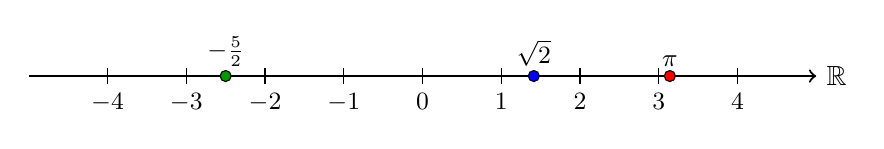
\begin{tikzpicture}
\draw[thick, ->] (-5,0) -- (5,0) node[right] {$\mathbb{R}$};
\foreach \x in {-4,-3,-2,-1,0,1,2,3,4}
    \draw (\x,0.1) -- (\x,-0.1) node[below] {\small $\x$};
\draw[fill=blue] (1.414,0) circle (2pt) node[above] {\small $\sqrt{2}$};
\draw[fill=red] (3.14159,0) circle (2pt) node[above] {\small $\pi$};
\draw[fill=green!60!black] (-2.5,0) circle (2pt) node[above] {\small $-\frac{5}{2}$};
\end{tikzpicture}
\end{center}

\begin{keypoint}
The hierarchy of number sets:
\[
\mathbb{N} \subset \mathbb{Z} \subset \mathbb{Q} \subset \mathbb{R}
\]
Natural numbers $\subset$ Integers $\subset$ Rationals $\subset$ Reals
\end{keypoint}

%-----------------------------------------------------------------------------
\section{Arithmetic with Real Numbers}
%-----------------------------------------------------------------------------

\subsection{Operations and Properties}

The four basic operations on real numbers are addition, subtraction, multiplication, and division.

\begin{formula}
\textbf{Properties of Real Number Arithmetic:}
\begin{align}
a + b &= b + a & ab &= ba & \text{(Commutative)}\\
(a + b) + c &= a + (b + c) & (ab)c &= a(bc) & \text{(Associative)}\\
a(b + c) &= ab + ac && & \text{(Distributive)}\\
a + 0 &= a & a \cdot 1 &= a & \text{(Identity)}\\
a + (-a) &= 0 & a \cdot \frac{1}{a} &= 1 \text{ (if } a \neq 0\text{)} & \text{(Inverse)}
\end{align}
\end{formula}

\subsection{Fractions}

\begin{formula}
\textbf{Fraction Operations:}
\begin{align}
\frac{a}{b} + \frac{c}{d} &= \frac{ad + bc}{bd} & \text{(Addition)}\\[2mm]
\frac{a}{b} - \frac{c}{d} &= \frac{ad - bc}{bd} & \text{(Subtraction)}\\[2mm]
\frac{a}{b} \times \frac{c}{d} &= \frac{ac}{bd} & \text{(Multiplication)}\\[2mm]
\frac{a}{b} \div \frac{c}{d} &= \frac{a}{b} \times \frac{d}{c} = \frac{ad}{bc} & \text{(Division)}
\end{align}
\end{formula}

\begin{example}
Simplify $\displaystyle \frac{2}{3} + \frac{3}{4}$.

\textbf{Solution:}
\[
\frac{2}{3} + \frac{3}{4} = \frac{2 \times 4 + 3 \times 3}{3 \times 4} = \frac{8 + 9}{12} = \frac{17}{12}
\]
\end{example}

\begin{example}
Simplify $\displaystyle \frac{5}{6} \div \frac{2}{9}$.

\textbf{Solution:}
\[
\frac{5}{6} \div \frac{2}{9} = \frac{5}{6} \times \frac{9}{2} = \frac{45}{12} = \frac{15}{4}
\]
\end{example}

\subsection{Order of Operations (PEMDAS/BODMAS)}

When evaluating expressions, follow this order:
\begin{enumerate}
    \item \textbf{P}arentheses / \textbf{B}rackets
    \item \textbf{E}xponents / \textbf{O}rders (powers, roots)
    \item \textbf{M}ultiplication and \textbf{D}ivision (left to right)
    \item \textbf{A}ddition and \textbf{S}ubtraction (left to right)
\end{enumerate}

\begin{example}
Evaluate $3 + 4 \times 2^2 - (6 - 2)$.

\textbf{Solution:}
\begin{align*}
3 + 4 \times 2^2 - (6 - 2) &= 3 + 4 \times 2^2 - 4 & \text{(parentheses)}\\
&= 3 + 4 \times 4 - 4 & \text{(exponent)}\\
&= 3 + 16 - 4 & \text{(multiplication)}\\
&= 15 & \text{(left to right)}
\end{align*}
\end{example}

%-----------------------------------------------------------------------------
\section{Inequalities and Intervals}
%-----------------------------------------------------------------------------

\subsection{Inequality Symbols}

\begin{center}
\begin{tabular}{|c|l|c|}
\hline
\textbf{Symbol} & \textbf{Meaning} & \textbf{Example} \\
\hline
$<$ & less than & $3 < 5$ \\
$>$ & greater than & $7 > 2$ \\
$\leq$ & less than or equal to & $x \leq 4$ \\
$\geq$ & greater than or equal to & $y \geq -1$ \\
$\neq$ & not equal to & $x \neq 0$ \\
\hline
\end{tabular}
\end{center}

\subsection{Properties of Inequalities}

\begin{property}[Rules for Inequalities]
For real numbers $a$, $b$, and $c$:
\begin{enumerate}
    \item \textbf{Addition/Subtraction:} If $a < b$, then $a + c < b + c$
    \item \textbf{Multiplication/Division by positive:} If $a < b$ and $c > 0$, then $ac < bc$
    \item \textbf{Multiplication/Division by negative:} If $a < b$ and $c < 0$, then $ac > bc$ (inequality reverses!)
\end{enumerate}
\end{property}

\begin{warning}
When multiplying or dividing an inequality by a \textbf{negative number}, you must \textbf{reverse} the inequality sign!
\end{warning}

\begin{example}
Solve $-2x + 3 < 7$.

\textbf{Solution:}
\begin{align*}
-2x + 3 &< 7\\
-2x &< 4 & \text{(subtract 3)}\\
x &> -2 & \text{(divide by $-2$, reverse inequality)}
\end{align*}
\end{example}

\subsection{Interval Notation}

Intervals describe sets of real numbers between two endpoints.

\begin{center}
\begin{tabular}{|c|c|c|}
\hline
\textbf{Interval} & \textbf{Inequality} & \textbf{Description} \\
\hline
$(a, b)$ & $a < x < b$ & Open interval (excludes $a$ and $b$) \\
$[a, b]$ & $a \leq x \leq b$ & Closed interval (includes $a$ and $b$) \\
$[a, b)$ & $a \leq x < b$ & Half-open (includes $a$, excludes $b$) \\
$(a, b]$ & $a < x \leq b$ & Half-open (excludes $a$, includes $b$) \\
$(a, \infty)$ & $x > a$ & All numbers greater than $a$ \\
$(-\infty, b]$ & $x \leq b$ & All numbers less than or equal to $b$ \\
$(-\infty, \infty)$ & $x \in \mathbb{R}$ & All real numbers \\
\hline
\end{tabular}
\end{center}

\begin{center}
\begin{tikzpicture}
\draw[thick, ->] (-1,0) -- (6,0);
\draw[thick, blue] (1,0) -- (4,0);
\draw[fill=white, draw=blue, thick] (1,0) circle (3pt);
\draw[fill=blue] (4,0) circle (3pt);
\node[below] at (1,-0.2) {$1$};
\node[below] at (4,-0.2) {$4$};
\node[above] at (2.5,0.2) {$(1, 4]$};
\end{tikzpicture}
\end{center}

\begin{example}
Express ``$x$ is at least $-3$ and less than $5$'' in interval notation.

\textbf{Solution:} $[-3, 5)$
\end{example}

%-----------------------------------------------------------------------------
\section{Absolute Value}
%-----------------------------------------------------------------------------

\begin{definition}[Absolute Value]
The \textbf{absolute value} of a real number $x$, written $|x|$, is its distance from 0 on the number line:
\[
|x| = \begin{cases}
x & \text{if } x \geq 0\\
-x & \text{if } x < 0
\end{cases}
\]
\end{definition}

\begin{example}
$|5| = 5$, $|-3| = 3$, $|0| = 0$
\end{example}

\begin{property}[Absolute Value Properties]
\begin{align}
|x| &\geq 0 \text{ always}\\
|xy| &= |x| \cdot |y|}\\
|x + y| &\leq |x| + |y| \text{ (Triangle Inequality)}
\end{align}
\end{property}

%=============================================================================
%=============================================================================
\chapter{Week 2: Linear Functions and Their Graphs}
%=============================================================================
%=============================================================================

\section{The Coordinate Plane}

\subsection{The Cartesian Plane}

\begin{definition}[Cartesian Coordinate System]
The \textbf{Cartesian plane} consists of two perpendicular number lines:
\begin{itemize}
    \item The horizontal \textbf{$x$-axis}
    \item The vertical \textbf{$y$-axis}
\end{itemize}
Their intersection is the \textbf{origin} $(0, 0)$.
\end{definition}

Every point in the plane is represented by an \textbf{ordered pair} $(x, y)$:
\begin{itemize}
    \item $x$ is the horizontal distance from the origin
    \item $y$ is the vertical distance from the origin
\end{itemize}

\begin{center}
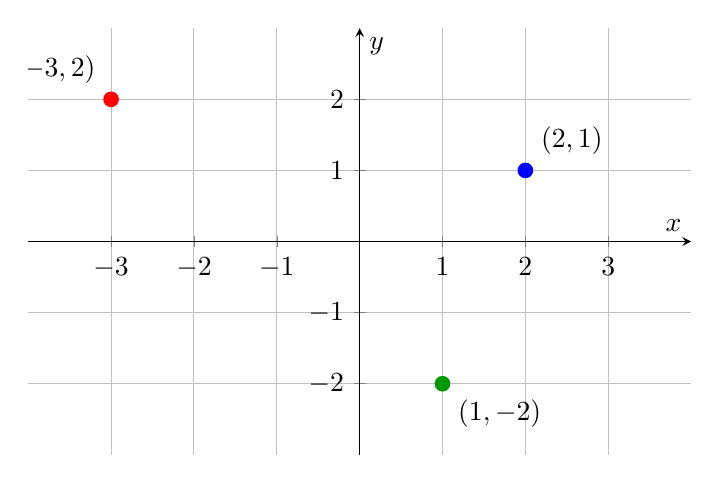
\begin{tikzpicture}
\begin{axis}[
    axis lines=middle,
    xlabel=$x$,
    ylabel=$y$,
    xmin=-4, xmax=4,
    ymin=-3, ymax=3,
    xtick={-3,-2,-1,1,2,3},
    ytick={-2,-1,1,2},
    grid=major,
    width=10cm,
    height=7cm
]
\node[circle,fill=blue,inner sep=2pt,label={above right:$(2,1)$}] at (axis cs:2,1) {};
\node[circle,fill=red,inner sep=2pt,label={above left:$(-3,2)$}] at (axis cs:-3,2) {};
\node[circle,fill=green!60!black,inner sep=2pt,label={below right:$(1,-2)$}] at (axis cs:1,-2) {};
\end{axis}
\end{tikzpicture}
\end{center}

\subsection{Quadrants}

The axes divide the plane into four \textbf{quadrants}:

\begin{center}
\begin{tabular}{|c|c|c|}
\hline
\textbf{Quadrant} & \textbf{Signs of $(x, y)$} & \textbf{Example} \\
\hline
I (upper right) & $(+, +)$ & $(3, 2)$ \\
II (upper left) & $(-, +)$ & $(-1, 4)$ \\
III (lower left) & $(-, -)$ & $(-2, -3)$ \\
IV (lower right) & $(+, -)$ & $(5, -1)$ \\
\hline
\end{tabular}
\end{center}

%-----------------------------------------------------------------------------
\section{Introduction to Functions}
%-----------------------------------------------------------------------------

\subsection{What is a Function?}

\begin{definition}[Function]
A \textbf{function} is a rule that assigns to each input value \textbf{exactly one} output value. If $f$ is a function and $x$ is an input, we write the output as $f(x)$ (read ``$f$ of $x$'').
\end{definition}

Think of a function as a machine:
\begin{center}
Input $x$ $\longrightarrow$ \fbox{Function $f$} $\longrightarrow$ Output $f(x)$
\end{center}

\begin{example}
Let $f(x) = 2x + 3$. Find $f(0)$, $f(2)$, and $f(-1)$.

\textbf{Solution:}
\begin{align*}
f(0) &= 2(0) + 3 = 3\\
f(2) &= 2(2) + 3 = 7\\
f(-1) &= 2(-1) + 3 = 1
\end{align*}
\end{example}

\begin{keypoint}
The key property of a function: each input has \textbf{exactly one} output. One input cannot produce two different outputs.
\end{keypoint}

\subsection{The Vertical Line Test}

\begin{property}[Vertical Line Test]
A graph represents a function if and only if every vertical line intersects the graph \textbf{at most once}.
\end{property}

\begin{center}
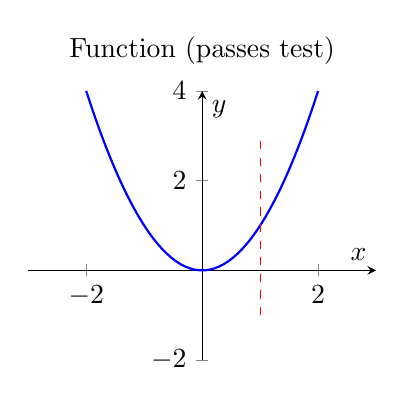
\begin{tikzpicture}
\begin{axis}[
    axis lines=middle,
    xlabel=$x$,
    ylabel=$y$,
    xmin=-3, xmax=3,
    ymin=-2, ymax=4,
    width=6cm,
    height=5cm,
    title={Function (passes test)}
]
\addplot[blue, thick, domain=-2:2, samples=50] {x^2};
\draw[dashed, red] (axis cs:1,-1) -- (axis cs:1,3);
\end{axis}
\end{tikzpicture}
\hspace{1cm}
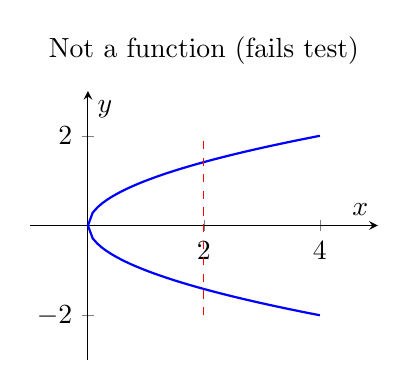
\begin{tikzpicture}
\begin{axis}[
    axis lines=middle,
    xlabel=$x$,
    ylabel=$y$,
    xmin=-1, xmax=5,
    ymin=-3, ymax=3,
    width=6cm,
    height=5cm,
    title={Not a function (fails test)}
]
\addplot[blue, thick, domain=0:4, samples=50] ({x},{sqrt(x)});
\addplot[blue, thick, domain=0:4, samples=50] ({x},{-sqrt(x)});
\draw[dashed, red] (axis cs:2,-2) -- (axis cs:2,2);
\end{axis}
\end{tikzpicture}
\end{center}

%-----------------------------------------------------------------------------
\section{Linear Functions}
%-----------------------------------------------------------------------------

\subsection{Definition and Forms}

\begin{definition}[Linear Function]
A \textbf{linear function} has the form:
\[
f(x) = mx + b
\]
where $m$ and $b$ are constants. Its graph is a straight line.
\end{definition}

\begin{formula}
\textbf{Forms of Linear Equations:}
\begin{align}
y &= mx + b & \text{(Slope-intercept form)}\\
y - y_1 &= m(x - x_1) & \text{(Point-slope form)}\\
ax + by &= c & \text{(Standard form)}
\end{align}
\end{formula}

\subsection{Slope}

\begin{definition}[Slope]
The \textbf{slope} of a line measures its steepness and direction:
\[
m = \frac{\text{rise}}{\text{run}} = \frac{y_2 - y_1}{x_2 - x_1} = \frac{\Delta y}{\Delta x}
\]
\end{definition}

\begin{center}
\begin{tabular}{|c|l|}
\hline
\textbf{Slope} & \textbf{Line Behavior} \\
\hline
$m > 0$ & Line rises from left to right \\
$m < 0$ & Line falls from left to right \\
$m = 0$ & Horizontal line \\
$m$ undefined & Vertical line \\
\hline
\end{tabular}
\end{center}

\begin{example}
Find the slope of the line through $(1, 2)$ and $(4, 8)$.

\textbf{Solution:}
\[
m = \frac{8 - 2}{4 - 1} = \frac{6}{3} = 2
\]
\end{example}

\subsection{$y$-intercept and $x$-intercept}

\begin{definition}[Intercepts]
\begin{itemize}
    \item The \textbf{$y$-intercept} is where the line crosses the $y$-axis (when $x = 0$).
    \item The \textbf{$x$-intercept} is where the line crosses the $x$-axis (when $y = 0$).
\end{itemize}
\end{definition}

For $y = mx + b$:
\begin{itemize}
    \item $y$-intercept: $(0, b)$
    \item $x$-intercept: $\left(-\frac{b}{m}, 0\right)$ (when $m \neq 0$)
\end{itemize}

\subsection{Graphing Linear Functions}

\begin{example}
Graph $f(x) = 2x - 3$.

\textbf{Solution:}
\begin{itemize}
    \item Slope: $m = 2$ (rise 2, run 1)
    \item $y$-intercept: $(0, -3)$
    \item $x$-intercept: Set $0 = 2x - 3 \Rightarrow x = \frac{3}{2}$, so $(\frac{3}{2}, 0)$
\end{itemize}

\begin{center}
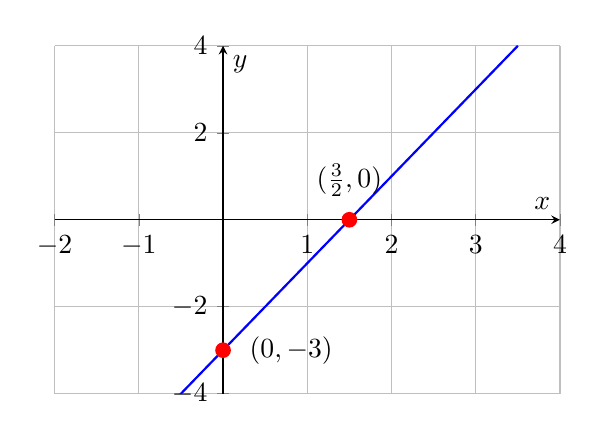
\begin{tikzpicture}
\begin{axis}[
    axis lines=middle,
    xlabel=$x$,
    ylabel=$y$,
    xmin=-2, xmax=4,
    ymin=-4, ymax=4,
    grid=major,
    width=8cm,
    height=6cm
]
\addplot[blue, thick, domain=-1:3.5] {2*x - 3};
\node[circle,fill=red,inner sep=2pt] at (axis cs:0,-3) {};
\node[circle,fill=red,inner sep=2pt] at (axis cs:1.5,0) {};
\node[right] at (axis cs:0.2,-3) {$(0,-3)$};
\node[above] at (axis cs:1.5,0.3) {$(\frac{3}{2},0)$};
\end{axis}
\end{tikzpicture}
\end{center}
\end{example}

%-----------------------------------------------------------------------------
\section{Solving Linear Equations}
%-----------------------------------------------------------------------------

\subsection{One-Variable Linear Equations}

\begin{example}
Solve $3x - 7 = 2x + 5$.

\textbf{Solution:}
\begin{align*}
3x - 7 &= 2x + 5\\
3x - 2x &= 5 + 7\\
x &= 12
\end{align*}
\end{example}

\subsection{Finding the Equation of a Line}

\begin{example}
Find the equation of the line through $(2, 5)$ with slope $3$.

\textbf{Solution:} Using point-slope form:
\begin{align*}
y - 5 &= 3(x - 2)\\
y - 5 &= 3x - 6\\
y &= 3x - 1
\end{align*}
\end{example}

\begin{example}
Find the equation of the line through $(1, 4)$ and $(3, 10)$.

\textbf{Solution:}
\begin{enumerate}
    \item Find slope: $m = \frac{10 - 4}{3 - 1} = \frac{6}{2} = 3$
    \item Use point-slope: $y - 4 = 3(x - 1)$
    \item Simplify: $y = 3x + 1$
\end{enumerate}
\end{example}

\subsection{Parallel and Perpendicular Lines}

\begin{property}[Parallel Lines]
Two lines are \textbf{parallel} if and only if they have the same slope: $m_1 = m_2$.
\end{property}

\begin{property}[Perpendicular Lines]
Two lines are \textbf{perpendicular} if and only if the product of their slopes is $-1$:
\[
m_1 \cdot m_2 = -1 \quad \text{or equivalently} \quad m_2 = -\frac{1}{m_1}
\]
\end{property}

\begin{example}
A line has slope $\frac{2}{3}$. What is the slope of a perpendicular line?

\textbf{Solution:} $m_\perp = -\frac{1}{2/3} = -\frac{3}{2}$
\end{example}

%=============================================================================
%=============================================================================
\chapter{Week 3: Polynomials and Their Graphs}
%=============================================================================
%=============================================================================

\section{Introduction to Polynomials}

\subsection{Definition}

\begin{definition}[Polynomial]
A \textbf{polynomial} in variable $x$ is an expression of the form:
\[
P(x) = a_n x^n + a_{n-1} x^{n-1} + \cdots + a_1 x + a_0
\]
where:
\begin{itemize}
    \item $a_n, a_{n-1}, \ldots, a_1, a_0$ are real numbers called \textbf{coefficients}
    \item $n$ is a non-negative integer
    \item $a_n \neq 0$ is the \textbf{leading coefficient}
    \item $n$ is the \textbf{degree} of the polynomial
    \item $a_0$ is the \textbf{constant term}
\end{itemize}
\end{definition}

\subsection{Classification by Degree}

\begin{center}
\begin{tabular}{|c|c|c|}
\hline
\textbf{Degree} & \textbf{Name} & \textbf{Example} \\
\hline
0 & Constant & $P(x) = 5$ \\
1 & Linear & $P(x) = 2x + 3$ \\
2 & Quadratic & $P(x) = x^2 - 4x + 4$ \\
3 & Cubic & $P(x) = x^3 - 1$ \\
4 & Quartic & $P(x) = x^4 + 2x^2 + 1$ \\
5 & Quintic & $P(x) = x^5 - x$ \\
\hline
\end{tabular}
\end{center}

\begin{example}
For $P(x) = 3x^4 - 2x^2 + 5x - 7$:
\begin{itemize}
    \item Degree: 4
    \item Leading coefficient: 3
    \item Constant term: $-7$
\end{itemize}
\end{example}

%-----------------------------------------------------------------------------
\section{Polynomial Operations}
%-----------------------------------------------------------------------------

\subsection{Addition and Subtraction}

Combine like terms (terms with the same power of $x$).

\begin{example}
Let $P(x) = 3x^3 + 2x^2 - x + 4$ and $Q(x) = x^3 - 5x^2 + 3$.

$P(x) + Q(x) = 4x^3 - 3x^2 - x + 7$

$P(x) - Q(x) = 2x^3 + 7x^2 - x + 1$
\end{example}

\subsection{Multiplication}

Distribute each term of one polynomial to every term of the other.

\begin{example}
$(2x + 3)(x^2 - x + 1)$
\begin{align*}
&= 2x(x^2 - x + 1) + 3(x^2 - x + 1)\\
&= 2x^3 - 2x^2 + 2x + 3x^2 - 3x + 3\\
&= 2x^3 + x^2 - x + 3
\end{align*}
\end{example}

\subsection{Special Products}

\begin{formula}
\textbf{Important Special Products:}
\begin{align}
(a + b)^2 &= a^2 + 2ab + b^2\\
(a - b)^2 &= a^2 - 2ab + b^2\\
(a + b)(a - b) &= a^2 - b^2\\
(a + b)^3 &= a^3 + 3a^2b + 3ab^2 + b^3\\
(a - b)^3 &= a^3 - 3a^2b + 3ab^2 - b^3
\end{align}
\end{formula}

%-----------------------------------------------------------------------------
\section{Quadratic Polynomials}
%-----------------------------------------------------------------------------

\subsection{Standard Form and Vertex Form}

\begin{definition}[Quadratic Function]
A \textbf{quadratic function} has the form:
\[
f(x) = ax^2 + bx + c \quad (a \neq 0)
\]
Its graph is a \textbf{parabola}.
\end{definition}

\begin{itemize}
    \item If $a > 0$: parabola opens \textbf{upward} (U-shape)
    \item If $a < 0$: parabola opens \textbf{downward} ($\cap$-shape)
\end{itemize}

\subsection{Solving Quadratic Equations}

\textbf{Method 1: Factoring}

\begin{example}
Solve $x^2 - 5x + 6 = 0$.

Factor: $(x - 2)(x - 3) = 0$

Solutions: $x = 2$ or $x = 3$
\end{example}

\textbf{Method 2: Quadratic Formula}

\begin{formula}
For $ax^2 + bx + c = 0$:
\[
x = \frac{-b \pm \sqrt{b^2 - 4ac}}{2a}
\]
\end{formula}

\begin{definition}[Discriminant]
The \textbf{discriminant} is $\Delta = b^2 - 4ac$:
\begin{itemize}
    \item $\Delta > 0$: Two distinct real roots
    \item $\Delta = 0$: One repeated real root
    \item $\Delta < 0$: No real roots (two complex roots)
\end{itemize}
\end{definition}

\begin{example}
Solve $2x^2 + 3x - 2 = 0$.

\textbf{Solution:}
\[
x = \frac{-3 \pm \sqrt{9 + 16}}{4} = \frac{-3 \pm 5}{4}
\]
$x = \frac{1}{2}$ or $x = -2$
\end{example}

\textbf{Method 3: Completing the Square}

\begin{example}
Solve $x^2 + 6x + 5 = 0$ by completing the square.

\begin{align*}
x^2 + 6x + 5 &= 0\\
x^2 + 6x &= -5\\
x^2 + 6x + 9 &= -5 + 9\\
(x + 3)^2 &= 4\\
x + 3 &= \pm 2\\
x &= -1 \text{ or } x = -5
\end{align*}
\end{example}

\subsection{Graphing Quadratics}

Key features of the parabola $y = ax^2 + bx + c$:

\begin{itemize}
    \item \textbf{Vertex}: $\left(-\frac{b}{2a}, f\left(-\frac{b}{2a}\right)\right)$
    \item \textbf{Axis of symmetry}: $x = -\frac{b}{2a}$
    \item \textbf{$y$-intercept}: $(0, c)$
    \item \textbf{$x$-intercepts}: Solutions to $ax^2 + bx + c = 0$ (if they exist)
\end{itemize}

\begin{example}
Graph $f(x) = x^2 - 4x + 3$.

\textbf{Analysis:}
\begin{itemize}
    \item Opens upward ($a = 1 > 0$)
    \item Vertex: $x = \frac{4}{2} = 2$, $y = 4 - 8 + 3 = -1$. Vertex: $(2, -1)$
    \item $y$-intercept: $(0, 3)$
    \item $x$-intercepts: $x^2 - 4x + 3 = (x-1)(x-3) = 0$, so $x = 1, 3$
\end{itemize}

\begin{center}
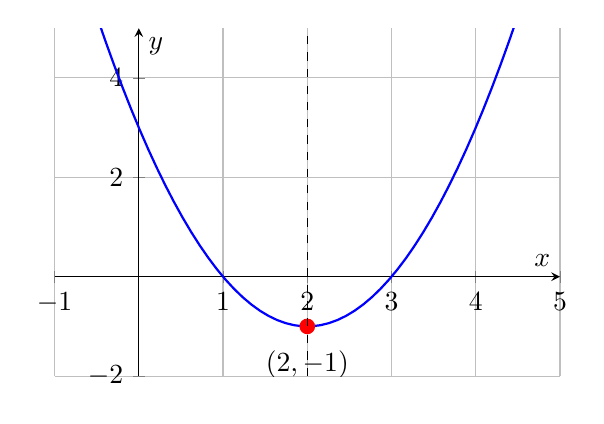
\begin{tikzpicture}
\begin{axis}[
    axis lines=middle,
    xlabel=$x$,
    ylabel=$y$,
    xmin=-1, xmax=5,
    ymin=-2, ymax=5,
    grid=major,
    width=8cm,
    height=6cm
]
\addplot[blue, thick, domain=-0.5:4.5, samples=50] {x^2 - 4*x + 3};
\node[circle,fill=red,inner sep=2pt] at (axis cs:2,-1) {};
\node[below] at (axis cs:2,-1.3) {$(2,-1)$};
\draw[dashed] (axis cs:2,-2) -- (axis cs:2,5);
\end{axis}
\end{tikzpicture}
\end{center}
\end{example}

%-----------------------------------------------------------------------------
\section{Graphs of Higher-Degree Polynomials}
%-----------------------------------------------------------------------------

\subsection{Roots (Zeros)}

\begin{definition}[Root/Zero]
A \textbf{root} (or \textbf{zero}) of polynomial $P(x)$ is a value $r$ such that $P(r) = 0$.
\end{definition}

A polynomial of degree $n$ has at most $n$ real roots.

\subsection{End Behavior}

The \textbf{end behavior} describes what happens to $P(x)$ as $x \to \pm\infty$.

\begin{center}
\begin{tabular}{|c|c|c|c|}
\hline
\textbf{Degree} & \textbf{Leading Coeff.} & \textbf{As $x \to -\infty$} & \textbf{As $x \to +\infty$} \\
\hline
Even & Positive & $+\infty$ & $+\infty$ \\
Even & Negative & $-\infty$ & $-\infty$ \\
Odd & Positive & $-\infty$ & $+\infty$ \\
Odd & Negative & $+\infty$ & $-\infty$ \\
\hline
\end{tabular}
\end{center}

\subsection{Turning Points}

\begin{definition}[Turning Point]
A \textbf{turning point} is where the graph changes from increasing to decreasing (local maximum) or from decreasing to increasing (local minimum).
\end{definition}

A polynomial of degree $n$ has at most $n - 1$ turning points.

\subsection{Multiplicity of Roots}

\begin{definition}[Multiplicity]
If $(x - r)^k$ is a factor of $P(x)$ but $(x - r)^{k+1}$ is not, then $r$ has \textbf{multiplicity} $k$.
\end{definition}

\begin{property}[Behavior at Roots]
At a root $r$ with multiplicity $k$:
\begin{itemize}
    \item $k$ odd: Graph \textbf{crosses} the $x$-axis
    \item $k$ even: Graph \textbf{touches} (bounces off) the $x$-axis
\end{itemize}
\end{property}

\begin{example}
Sketch $P(x) = (x + 1)^2(x - 2)$.

\textbf{Analysis:}
\begin{itemize}
    \item Degree: 3 (odd), leading coefficient: positive
    \item End behavior: $-\infty$ to $+\infty$
    \item Roots: $x = -1$ (multiplicity 2, bounces), $x = 2$ (multiplicity 1, crosses)
    \item $y$-intercept: $P(0) = 1 \cdot (-2) = -2$
\end{itemize}

\begin{center}
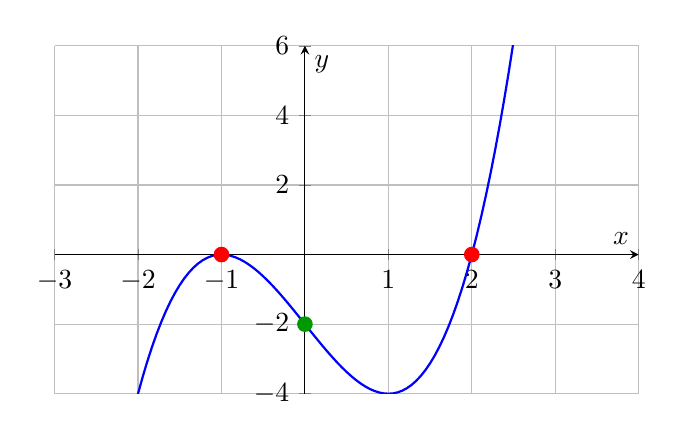
\begin{tikzpicture}
\begin{axis}[
    axis lines=middle,
    xlabel=$x$,
    ylabel=$y$,
    xmin=-3, xmax=4,
    ymin=-4, ymax=6,
    grid=major,
    width=9cm,
    height=6cm
]
\addplot[blue, thick, domain=-2.5:3, samples=100] {(x+1)^2*(x-2)};
\node[circle,fill=red,inner sep=2pt] at (axis cs:-1,0) {};
\node[circle,fill=red,inner sep=2pt] at (axis cs:2,0) {};
\node[circle,fill=green!60!black,inner sep=2pt] at (axis cs:0,-2) {};
\end{axis}
\end{tikzpicture}
\end{center}
\end{example}

%=============================================================================
%=============================================================================
\chapter{Week 4: Functions and Graphs}
%=============================================================================
%=============================================================================

\section{Domain and Range}

\subsection{Definitions}

\begin{definition}[Domain]
The \textbf{domain} of a function is the set of all valid input values.
\end{definition}

\begin{definition}[Range]
The \textbf{range} of a function is the set of all possible output values.
\end{definition}

\subsection{Finding Domain}

For most functions, find values where the function is undefined:
\begin{itemize}
    \item \textbf{Division by zero}: Exclude values making denominator zero
    \item \textbf{Square roots of negatives}: Exclude values making radicand negative
    \item \textbf{Polynomials}: Domain is all real numbers $\mathbb{R}$
\end{itemize}

\begin{example}
Find the domain of $f(x) = \frac{1}{x - 3}$.

\textbf{Solution:} Undefined when $x - 3 = 0$, i.e., $x = 3$.

Domain: $\{x \in \mathbb{R} : x \neq 3\}$ or $(-\infty, 3) \cup (3, \infty)$
\end{example}

\begin{example}
Find the domain of $g(x) = \sqrt{x - 2}$.

\textbf{Solution:} Requires $x - 2 \geq 0$, i.e., $x \geq 2$.

Domain: $[2, \infty)$
\end{example}

\subsection{Finding Range from Graphs}

The range is the set of $y$-values covered by the graph.

\begin{example}
For $f(x) = x^2$:
\begin{itemize}
    \item Domain: $(-\infty, \infty)$
    \item Range: $[0, \infty)$ (parabola has minimum at $y = 0$)
\end{itemize}
\end{example}

%-----------------------------------------------------------------------------
\section{Properties of Functions from Graphs}
%-----------------------------------------------------------------------------

\subsection{Increasing and Decreasing}

\begin{definition}[Increasing/Decreasing]
A function $f$ is:
\begin{itemize}
    \item \textbf{Increasing} on an interval if $f(x_1) < f(x_2)$ whenever $x_1 < x_2$
    \item \textbf{Decreasing} on an interval if $f(x_1) > f(x_2)$ whenever $x_1 < x_2$
\end{itemize}
\end{definition}

Visually:
\begin{itemize}
    \item Increasing: graph goes \textbf{up} as you move right
    \item Decreasing: graph goes \textbf{down} as you move right
\end{itemize}

\subsection{Positive and Negative Regions}

\begin{itemize}
    \item $f(x) > 0$: graph is \textbf{above} the $x$-axis
    \item $f(x) < 0$: graph is \textbf{below} the $x$-axis
    \item $f(x) = 0$: graph is \textbf{on} the $x$-axis (roots)
\end{itemize}

\subsection{Local Extrema}

\begin{definition}[Local Maximum/Minimum]
\begin{itemize}
    \item A \textbf{local maximum} occurs at $x = c$ if $f(c) \geq f(x)$ for all $x$ near $c$
    \item A \textbf{local minimum} occurs at $x = c$ if $f(c) \leq f(x)$ for all $x$ near $c$
\end{itemize}
\end{definition}

%-----------------------------------------------------------------------------
\section{Continuity}
%-----------------------------------------------------------------------------

\subsection{Intuitive Understanding}

\begin{definition}[Continuous Function]
A function is \textbf{continuous} if you can draw its graph without lifting your pen. There are no breaks, holes, or jumps.
\end{definition}

\begin{property}[Polynomials are Continuous]
Every polynomial function is continuous on $(-\infty, \infty)$.
\end{property}

\subsection{Types of Discontinuities}

\begin{center}
\begin{tabular}{|c|l|}
\hline
\textbf{Type} & \textbf{Description} \\
\hline
Removable (hole) & Single point missing from graph \\
Jump & Graph ``jumps'' from one value to another \\
Infinite (asymptote) & Graph approaches $\pm\infty$ \\
\hline
\end{tabular}
\end{center}

\begin{example}
$f(x) = \frac{1}{x}$ has an infinite discontinuity at $x = 0$.

$g(x) = \frac{x^2 - 1}{x - 1}$ has a removable discontinuity (hole) at $x = 1$.
\end{example}

%-----------------------------------------------------------------------------
\section{Building New Functions}
%-----------------------------------------------------------------------------

\subsection{Arithmetic Operations}

Given functions $f$ and $g$:

\begin{formula}
\begin{align}
(f + g)(x) &= f(x) + g(x)\\
(f - g)(x) &= f(x) - g(x)\\
(f \cdot g)(x) &= f(x) \cdot g(x)\\
\left(\frac{f}{g}\right)(x) &= \frac{f(x)}{g(x)} \quad (g(x) \neq 0)
\end{align}
\end{formula}

\begin{example}
Let $f(x) = x^2$ and $g(x) = x + 1$.
\begin{itemize}
    \item $(f + g)(x) = x^2 + x + 1$
    \item $(f \cdot g)(x) = x^2(x + 1) = x^3 + x^2$
    \item $\left(\frac{f}{g}\right)(x) = \frac{x^2}{x + 1}$ (domain: $x \neq -1$)
\end{itemize}
\end{example}

\subsection{Composition of Functions}

\begin{definition}[Composition]
The \textbf{composition} of $f$ and $g$, written $(f \circ g)(x)$ or $f(g(x))$, means ``apply $g$ first, then apply $f$ to the result.''
\[
(f \circ g)(x) = f(g(x))
\]
\end{definition}

\begin{keypoint}
Order matters! In general, $f \circ g \neq g \circ f$.
\end{keypoint}

\begin{example}
Let $f(x) = x^2$ and $g(x) = x + 3$.

$(f \circ g)(x) = f(g(x)) = f(x + 3) = (x + 3)^2 = x^2 + 6x + 9$

$(g \circ f)(x) = g(f(x)) = g(x^2) = x^2 + 3$

Note: $(f \circ g)(x) \neq (g \circ f)(x)$
\end{example}

\begin{example}
Let $f(x) = \sqrt{x}$ and $g(x) = x - 4$.

Find $(f \circ g)(x)$ and its domain.

\textbf{Solution:}
$(f \circ g)(x) = f(g(x)) = f(x - 4) = \sqrt{x - 4}$

Domain: Need $x - 4 \geq 0$, so $x \geq 4$. Domain: $[4, \infty)$
\end{example}

\subsection{Domain of Composite Functions}

The domain of $f \circ g$ consists of all $x$ in the domain of $g$ such that $g(x)$ is in the domain of $f$.

%-----------------------------------------------------------------------------
\section{Transformations of Functions}
%-----------------------------------------------------------------------------

\subsection{Vertical and Horizontal Shifts}

\begin{center}
\begin{tabular}{|c|l|}
\hline
\textbf{Transformation} & \textbf{Effect on Graph} \\
\hline
$f(x) + k$ & Shift \textbf{up} by $k$ units \\
$f(x) - k$ & Shift \textbf{down} by $k$ units \\
$f(x - h)$ & Shift \textbf{right} by $h$ units \\
$f(x + h)$ & Shift \textbf{left} by $h$ units \\
\hline
\end{tabular}
\end{center}

\subsection{Reflections and Stretches}

\begin{center}
\begin{tabular}{|c|l|}
\hline
\textbf{Transformation} & \textbf{Effect on Graph} \\
\hline
$-f(x)$ & Reflect across $x$-axis \\
$f(-x)$ & Reflect across $y$-axis \\
$af(x)$ ($a > 1$) & Vertical stretch by factor $a$ \\
$af(x)$ ($0 < a < 1$) & Vertical compression by factor $a$ \\
\hline
\end{tabular}
\end{center}

\begin{example}
Starting with $f(x) = x^2$, describe the graph of $g(x) = -(x - 2)^2 + 3$.

\textbf{Transformations:}
\begin{enumerate}
    \item Start with $y = x^2$
    \item Shift right 2 units: $y = (x-2)^2$
    \item Reflect across $x$-axis: $y = -(x-2)^2$
    \item Shift up 3 units: $y = -(x-2)^2 + 3$
\end{enumerate}

Result: Parabola opening downward with vertex at $(2, 3)$.
\end{example}

%=============================================================================
\chapter*{Summary}
\addcontentsline{toc}{chapter}{Summary}
%=============================================================================

\section*{Week 1: Numbers}
\begin{itemize}
    \item Number sets: $\mathbb{N} \subset \mathbb{Z} \subset \mathbb{Q} \subset \mathbb{R}$
    \item Rational numbers have terminating or repeating decimals
    \item Inequalities: reverse sign when multiplying/dividing by negative
    \item Interval notation: $(a,b)$, $[a,b]$, $(a,b]$, $[a,b)$
\end{itemize}

\section*{Week 2: Linear Functions}
\begin{itemize}
    \item Slope: $m = \frac{y_2 - y_1}{x_2 - x_1}$
    \item Slope-intercept form: $y = mx + b$
    \item Point-slope form: $y - y_1 = m(x - x_1)$
    \item Parallel lines: same slope; Perpendicular lines: $m_1 \cdot m_2 = -1$
\end{itemize}

\section*{Week 3: Polynomials}
\begin{itemize}
    \item Degree $n$ polynomial: at most $n$ roots and $n-1$ turning points
    \item Quadratic formula: $x = \frac{-b \pm \sqrt{b^2 - 4ac}}{2a}$
    \item Discriminant $\Delta = b^2 - 4ac$ determines nature of roots
    \item End behavior depends on degree (odd/even) and leading coefficient sign
    \item Root multiplicity: odd = crosses, even = bounces
\end{itemize}

\section*{Week 4: Functions and Graphs}
\begin{itemize}
    \item Domain: valid inputs; Range: possible outputs
    \item Polynomials are continuous everywhere
    \item Composition: $(f \circ g)(x) = f(g(x))$
    \item Transformations: shifts, reflections, stretches
\end{itemize}

\end{document}
